\documentclass[spanish]{article}
\usepackage[spanish]{babel}
\usepackage{amsmath}
\usepackage{amssymb}
\usepackage[utf8]{inputenc}
\usepackage{vmargin}
\usepackage{graphicx}
\usepackage{wrapfig}
\usepackage[export]{adjustbox}


\begin{document}

	\setpapersize{USletter}
	\setmarginsrb{30mm}{30mm}{30mm}{30mm}{0pt}{0mm}{0pt}{0mm}
	
	\begin{center}
	{\Large Análisis de Algoritmos, Sem: 2018-1, 3CV2 Práctica 2, 7 de Septiembre del 2017}\\
{\huge {\bf Práctica 3: Divide y Venceras: Algoritmo Merge Sort.}} \\
{\large {\bf Luis Daniel Martinez Berumen}}\\
	
\includegraphics[width=1\textwidth]{./imagenes/logos.png}\\
	\end{center}
	\bigskip
	\bigskip
	\bigskip
	{\LARGE {\bf Abstract}}\\
En esta practica vamos a demostrar tanto de manera analitica como de manera practica, con graficas de los experimentos, la complejidad de dos algoritmos de ordenamiento, Merge y MergeSort, siendo el primero de complejidad lineal y el segundo de complejidad $\theta$(n log (n)).\\
Valiendonos del paradigma de "Divide y venceras", el cual nos ayudara a simplificar el trabajo. Ademas de mostrar la resolucion de 2 problemas con propiedades de los algoritmos vistos en clase.\\\\\\
	{\Large {\bf Palabras Clave}}
	\begin{itemize}
		\item Algoritmo
		\item Fucion
		\item Recursividad
		\item Paradigma
		\item Dividir
	\end{itemize}
	
	\section{Introducci\'on}
	Divide y Vencerás es una frase quye hemos escuchado todos, al menos, una vez en nuestra vida, para nosotros 
	es técnica de diseño de algoritmos, siendo de gran utilidad para nuestra carrera, ya que, 
	los problemas a los que nos enfrentamos día con día son mas faciles de resolver si aplciamos una tecnica de este tipo.
	De hecho, suele ser considerada una filosofía general para resolver problemas, no solo del termino informatico, sino que también se utiliza en muchos otros ámbitos


\newpage
	\section{Conceptos B\'asicos}
	Para la correcta comprension de este trabajo, es necesario definir algunos terminos tales como $\theta$, O y $\Omega$.\\
	 $\theta$(n):\\
		Sea g(n) una función. Se define  $\theta$ (g(n)) como:\\
		
		 	$\theta$(g(n)) = $\{ f(n) \quad | \quad \exists c1,c2>0 \quad \& \quad n_{0}>0 \quad \mid \quad \forall n>=n_{0} \quad 0<= c1g(n) <= f(n) <= c2g(n) \}$
	\bigskip		 	
		 	
	O(n):\\
		Sea  g(n)  una función, O(n) (el pero de los casos) se define como:\\
		
			\hspace{1cm}O(n)=$\{f(n) \quad | \quad \exists c >0 \quad \& \quad n_{0}>0 \quad | \quad f(n) <= Cg(n) \quad \forall  n>= n_{0} \}$
	\bigskip
	
	$\Omega$(n):\\
	Sea  g(n)  una función. Se define $\Omega$ (g(n)) (el mejor de los casos) como:\\

		\hspace{1cm}$\Omega$(g(n)) =$\{f(n) \quad | \quad \exists c >0 \quad \& \quad n_{0}>0 \quad \mid \quad  0<= cg(n)<= f(n) \quad \forall n>= n_{0} \}$
	\bigskip

	El algoritmo de MergeSort es un método de ordenamiento por mezcla, la idea general es que: Dados dos conjuntos ordenados, A y B, si los mezclamos entre ambos, tomando los valores de ellos en orden, entonces nos devolvera el conjunto ordenado C, con los elementos de A y B.
	\bigskip
	Partiendo de este punto, aplicaremos la estrategia Divide y Vencerás. La idea es, que si inicialmente tenemos la lista desordenada, y la dividimos a la mitad, nos quedaremos con 2 sub-listas desordenadas, entonces, realizamos otra vez la misma acción: dividimos las sub-listas resultantes en 4 nuevas sub-listas, y así sucesivamente.
	\bigskip
	Esta operación se realizará hasta que lleguemos a una sub-lista con 1  elemento en ella, que por defecto va a estar ordenada, y como dicha sub-lista ya está ordenada, la mezclamos con la de al lado, que está ordenada también, y así continuamente vamos ordenando las sub-listas hacia arriba para llegar al caso base.

	\bigskip
	Si representamos esas operaciones en una imagen, puedes notar que se forma un árbol, donde, partiendo de las hojas (son los elementos terminales del árbol), se van a ordenar los nodos padres, por medio de la mezcla entre sus dos hijos, hasta llegar al nodo raíz.\\

	\begin{center}
	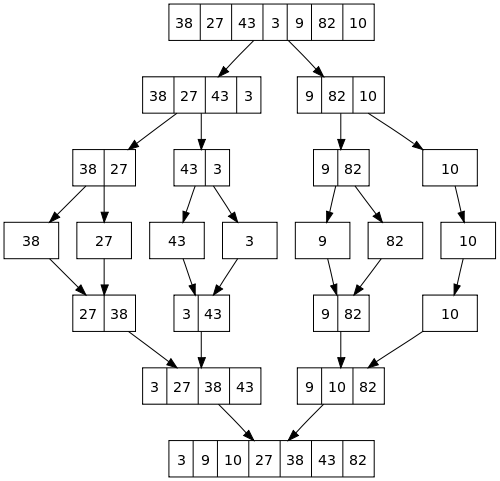
\includegraphics[width=100mm]{./imagenes/i1.png}\\
		Figura 1: Arbol 
	\end{center}
	\newpage	

	\bigskip
	\section{Experimentaci\'on y Resultados}
	
	\subsection{Implemente el algortimo MergeSort}
	
	{\large{\bf i)Mediante graficas, muestre que el algoritmo Merge tiene complejidad lineal.}}\\
	Colocando un contador para cada vez que se llama a la funcion merge, la cual se ejecuta para cada uno de los elementos de nustro arreglo, se obtubo la siguiente grafica:\\
	\begin{center}
	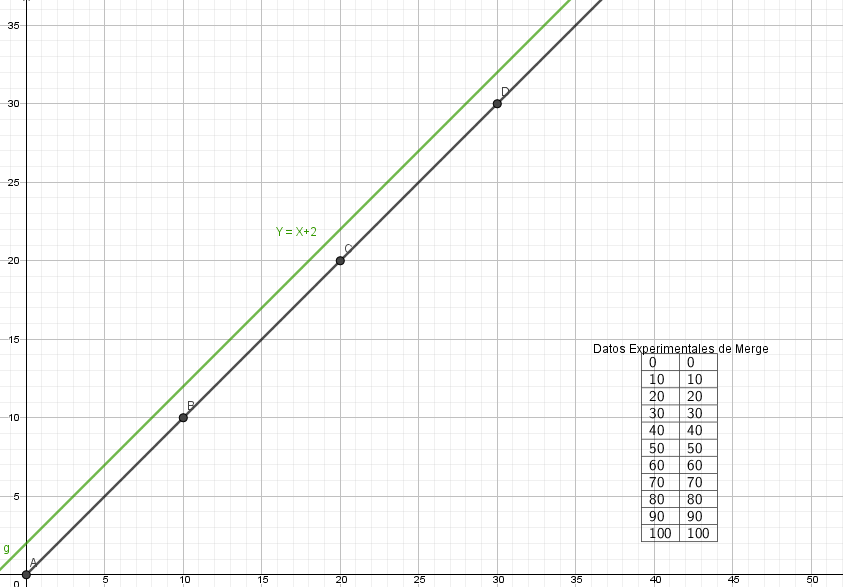
\includegraphics[scale=.5]{./imagenes/merge.png}\\
		Figura 2: Complejidad del algoritmo Merge mediante graficas
	\end{center}
	Por lo siguiente, debido a que para cada uno de los elementos la funcion Merge es llamada una vez, y cortejandola con una funcion del tipo:  $\theta$ (n) se concluye que la complejidad del algoritmo Merge es lineal.\\

	\newpage
	{\large{\bf ii)Demostrar analiticamente que el algortimo Merge tiene complejidad lineal.}}\\
		merge(A, p, q, r)  \hspace{4cm} Costo \hspace{4cm} Pasos\\
	1.- n1 $\leftarrow$ p-q+1\hspace{4.5cm} C1 \hspace{5cm} 1 \\
	2.- n2 $\leftarrow$ r-q\hspace{5.1cm} C2 \hspace{5cm} 1\\
	4.- for i=0 to i$<$n1 do:\hspace{3.3cm} C3 \hspace{5cm} n \\
	5.- \hspace{0.7cm}L[ i ] $\leftarrow$ A[ p+i ]  \hspace{2.9cm} C4 \hspace{5cm} n-1 \\
	6.- for j=0 to i$<$n2 do:\hspace{3.3cm} C5 \hspace{5cm} n \\
	7.- \hspace{0.7cm}R[ j ] $\leftarrow$ A[ q+1+j ]  \hspace{2.3cm} C6 \hspace{5cm} n-1 \\
	8.- i $\leftarrow$ 0\hspace{5.8cm} C7 \hspace{5cm} 1 \\
	9.- j $\leftarrow$ 0\hspace{5.8cm} C8 \hspace{5cm} 1\\
	10.- for k=p to k$<$r do:\hspace{3.2cm} C9 \hspace{5cm} n \\
	11.- \hspace{0.5cm}if L[ i ]$<$R[ j ]  \hspace{3.5cm} C10 \hspace{4.8cm} n-1 \\
	12.-\hspace{1cm} A[ k ]=L[ j ] \hspace{3.3cm} C11 \hspace{4.8cm} n-1\\
	13.- \hspace{1cm} i++ \hspace{4.6cm} C12 \hspace{4.8cm} n-1\\
	14.- \hspace{0.5cm}else  \hspace{5.5cm} C13 \hspace{4.8cm} n-1\\
	15.-\hspace{1cm} A[ k ]=R[ j ] \hspace{3.3cm} C14 \hspace{4.8cm} n-1\\
	16.- \hspace{1cm} j++ \hspace{4.6cm} C15 \hspace{4.8cm} n-1\\
	8.- return a\hspace{5.5cm} C16 \hspace{4.8cm} 1 \\\\

    \noindent {\bf Demostración.}\\
	Tenemos que:\\
	T(n) = C1 + C2 + C3n + C4(n-1) + C5n + C6(n-1) + C7 + C8 + C9n + C10(n-1) + C11(n-1) + C12(n-1) + C13(n-1) + C14(n-1) + C15(n-1) + C16\\
	T(n) = C1 + C2 + C3n + C4n - C4 + C5n + C6n - C6 + C7 + C8 + C9n + C10n - C10 + C11n - C11 + C12n - C12 + C13n - C13 + C14n - C14 + C15n - C15 + C16\\
	Al factorizar nos queda:\\
	T(n) = (C3 + C4 + C5 + C6 + C7 + C9 + C10 + C11 + C12 + C13 + C14)n + (C1 + C2 + + C7 + C8 + C16 - C4 - C6 - C10 - C11 - C12 - C13 - C14 - C16)\\
	$\therefore$\\
	T(n) $\in$ $\theta$(n)\\
	
	\newpage
	{\large{\bf  iii)Mostrar mediante graficas, que el algoritmo MergeSort tiene complejidad $\theta$ (nlogn).}}\\
	Colocando un contador para cada vez que se llama a la funcion mergeSort, la cual se ejecuta para cada uno de los elementos de nustro arreglo, se obtubo la siguiente tabla:\\
	\begin{center}
	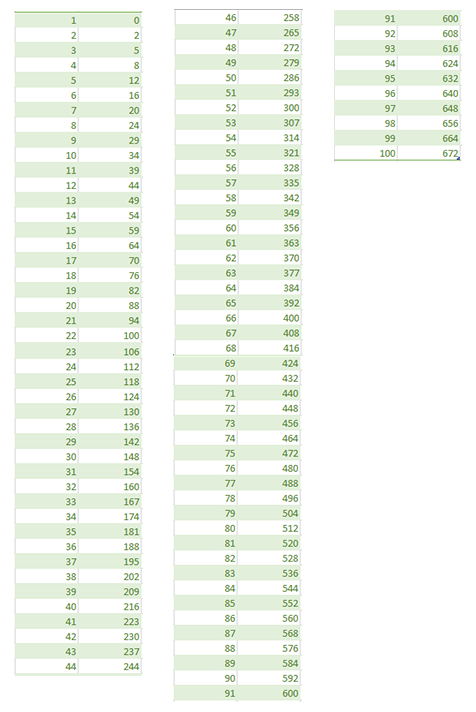
\includegraphics[scale=.5]{./imagenes/tablas.png}\\
		Figura 3: Resultados obtenidos tras la ejecucion de MergeSort
	\end{center}
	Para este algoritmo se propone la funcion $\theta$(nlog(n)), quedando graficada de color verde, siendo la linea de color obscuro, la grafica de la tabla anterior.
	\begin{center}
	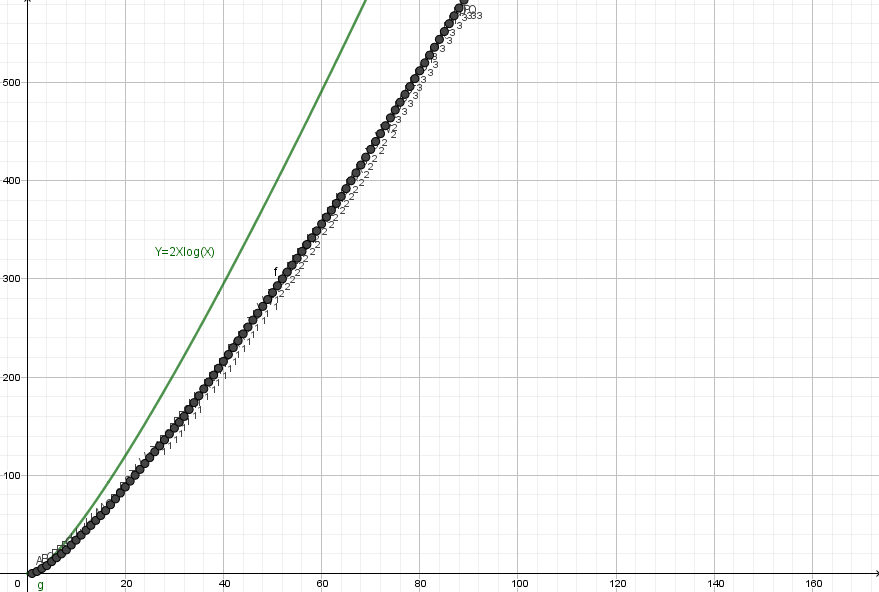
\includegraphics[scale=.5]{./imagenes/mergesort.png}\\
		Figura 4: Complejidad del algoritmo MergeSort mediante graficas.
	\end{center}
	Debido a los resultados obtendidos tras la experimentacion, se concluye que el algoritmo MergeSort, tiene complejidad nlog(n)


	\newpage
	{\large{\bf  iv)Demostrar analiticamente que el algoritmo MergeSort tiene complejidad $\theta$ (nlogn). }}\\		
	\noindent mergesort(A, p, r)  \hspace{4cm} Costo\\
	1.- if p$<$r \hspace{5.6cm} 1\\
    2.- q = $\frac{(p + r)}{2}$ \hspace{5cm} D( n )\\
    3.- Mergesort(A, p, q) \hspace{3.3cm} T( $\frac{n}{2}$ )\\
    4.- Mergesort(A, q+1, r) \hspace{2.8cm} T( $\frac{n}{2}$ )\\
    5.- Merge (A, p, q, r) \hspace{3.4cm} C( n )\\
    
    \noindent Sea D( n ) el costo computacional de dividir el arreglo de tamaño n.\\
    \noindent Sea C( n ) el costo computacional de combinar l a solución de subproblemas para obtener la solución del problema original.\\
    luego\\
    \begin{equation}
        T( n )=\left \{ 
            \begin{array}{lcc}
            \theta & si & n=1\\
            2T( \frac{n}{2} )+D( n )+C( n ) & si & n>1
            \end{array}
        \right.  
    \end{equation}
    \newline
    \begin{equation}
    T( n )=\left \{ 
            \begin{array}{lcc}
            C_1 & si & n=1\\
            2T( \frac{n}{2} )+\theta( n ) & si & n>1
            \end{array}
        \right.
    \end{equation}
    \newline
    \begin{equation}
        T( n )=\left \{ 
            \begin{array}{lcc}
            C & si & n=1\\
            2T( \frac{n}{2} )+C_n & si & n>1
            \end{array}
        \right.
    \end{equation}
    \newline 
    \noindent Sea n tal que K=$\log_2$n (n=$2^K$) luego\\
    C si n=$2^k$=1\\
    2T( $2^{k-1}$ )+C$2^k$ si n=$2^n>$1\\
    T( $2^{K-1}$ )=2T( $2^{K-1}$ )+$2^K$\\
    =2[ 2T( $2^K-2$ )+C$2^{K-1}$ ]C$2^K$\\
    ...\\
    =$2^{i}$T( $2^{K-i}$ )+iC$2^K$ k-i=0 k=i\\
    =$2^K$T( 1 )+KC$2^K$\\
    =C$2^K$+K$2^K$\\
    =(K+1)C$2^K$\\
    =$\log_2$(n+1)Cn\\
    =Cn$\log_2$n+Cn $\in \theta$ ( n$\log_2$n ) 

\newpage

\newpage
\section{Conclusi\'on}

	\bigskip
	En esta practica logre darme cuenta que ordenar un arreglo es mas complejo de lo que parece, que es nuestro deber saber implementar bien cada uno de los algoritmos que vamos conociendo
	para así lograr obtener el mejor resultado, al principio tuve algunos problemas con las graficas, debido a que no sabia que el MergeSort era logaritmico, yo pense que sería exponencial, 
	me agrado lograr determinar despues que sun complejidad es logartimica ya que eso era lo que indicaban mis resultado.\\
	De igual manera me parece que el escoger Python para programar estos ejercicios fue la desicion correcta, es mas sencillo trabajar con los datos en este lenguaje y asi obtener los resultados esperados.
	\bigskip


	\section{Anexos:}
	
	\subsection{Calcular el orden de complejidad de los siguientes algoritmos en el mejor ($\Omega$) y en el peor de los casos (O) (no es necesario hacer el analisis linea por linea, en este 		caso, puede aplicar propiedades de los algoritmos vistos en clase):}

	{\large{A}}\\

	Función1( n par )\\
	1. i=0\\
	2. mientras i < n hacer\\
	3. \hspace{0.5cm} para j=1 hasta j=10 hacer\\
	4. \hspace{1.0cm} Accion(i) \\
	5. 	\hspace{1.0cm} j++\\
	6. i+=2\\
	Suponga que Accion $\in$  $\theta$(1)\\
	\bigskip
	Solución\\
	A) 1.i=0 $\leftarrow$ $\theta$(1)\\
	B) 2. mientras i<n hacer $\leftarrow$ $\theta$(n)\\
	C) 3.\hspace{0.5cm} para j=1 hasta j=10 $\leftarrow$ $\theta$(n)\\
	D) por el teorema 1.4 para 2. y 3. $\leftarrow$ $\theta$($n^{2}$)\\
	E) 4.\hspace{1.0cm} Accion(i) $\leftarrow$ $\theta$(1)\\
	F) 5.\hspace{1.0cm} j++  $\leftarrow$ $\theta$(1)\\
	G) 6. i+=2 $\leftarrow$ $\theta$(1)\\
	H) $T(n) = \theta(1) + \theta(n^{2})  + \theta(1) + \theta(1) + \theta(1)
		= \theta(1) + + \theta(n^{2}) $\\
		Por los teoremas 1.2 y 1.4 :\\
		$T(n) = \theta(n^{2})$ \\
	

\newpage
	{\large{B}}\\

	Función2(A[0,....n-1,x entero])\\
	1. for i=0 to i<n do\\
	2. \hspace{0.5cm} if(A[i]<x)\\
	3.  \hspace{1.0cm} A[i]=min(A[0,....n-1])\\
	4. \hspace{0.5cm} else if(A[i]>x) \\
	5. \hspace{1.0cm} A[i]=max(A[0,....n-1])\\
	6. \hspace{0.5cm} else\\
	7.\hspace{1.0cm} exit\\
	Solución\\
	En el mejor de los casos es cuando  A[i]=X, lo cual deja   $T(n) = \theta(1)$ \\
	El peor de los casos es cuando A[i]!=x , por lo que \\
	A) 1. $ for \quad i =0 \quad i< n \quad do \leftarrow \theta (n)\\ $
	B) 2. $ \hspace{0.5cm} if(A[i]<x) \leftarrow \theta(1)\\$
	C) 3. $ \hspace{1.0cm} A[i]=min(A[0,....n-1]) \leftarrow \theta(n)\\$
	D)$ \hspace{1.3cm} Por\quad el \quad teorema \quad 1.4 \quad en \quad 2.\quad  y\quad  .3 \quad \leftarrow \theta(n)\\$
	E) 4. $\hspace{0.5cm} elseif \quad (A[i]>X) \leftarrow \theta(1)\\ $
	F) 5. $\hspace{1.0cm} A[i]=max(A[0,....n-1]) \leftarrow \theta(n)\\$
	G)$ \hspace{1.3cm} Por \quad  el \quad  teorema \quad   1.4 \quad en \quad   4. \quad   y \quad  .5 \quad b\leftarrow \theta(n)\\$
	H) 6. $\hspace{50mm} else \quad  \leftarrow \theta(1).\\$
	I) 7. $\hspace{0.5cm}  exit \quad \leftarrow \theta(1)\\$
	j)$ \hspace{1.3cm} Por \quad \quad el \quad teorema \quad  1.2 \quad en \quad 6. \quad  y .7 \quad \leftarrow \theta(1)\\$
	$T(n) = \theta(n) + \theta(n)  + \theta(n) + \theta(1) $\\
		Por los teoremas 1.2 y 1.4 :\\
		$T(n) = \theta(n)$ \\
		\bigskip
\end{document}